\documentclass[12pt,a4paper]{article}
\usepackage{float}
\usepackage{amsmath,amscd,amsbsy,amssymb,latexsym,url,bm,amsthm}
\usepackage{epsfig,graphicx,subfigure}
\usepackage{enumitem,balance,mathtools}
\usepackage{wrapfig}
\usepackage{mathrsfs, euscript}
\usepackage[usenames]{xcolor}
\usepackage{hyperref}
\usepackage{comment}
\usepackage[T1]{fontenc}
\usepackage{algorithmic}
\usepackage[ruled,lined,boxed,linesnumbered]{algorithm2e}
\usepackage{xcolor}
\usepackage{listings}
\usepackage{indentfirst}


\floatname{algorithm}{Solution}
\newtheorem{theorem}{Theorem}[section]
\newtheorem{lemma}[theorem]{Lemma}
\newtheorem{proposition}[theorem]{Proposition}
\newtheorem{corollary}[theorem]{Corollary}
\newtheorem{exercise}{Exercise}[section]
\newtheorem*{solution}{Solution}

\renewcommand{\thefootnote}{\fnsymbol{footnote}}

\newcommand{\postscript}[2]
 {\setlength{\epsfxsize}{#2\hsize}
  \centerline{\epsfbox{#1}}}

\renewcommand{\baselinestretch}{1.0}

\setlength{\oddsidemargin}{-0.365in}
\setlength{\evensidemargin}{-0.365in}
\setlength{\topmargin}{-0.3in}
\setlength{\headheight}{0in}
\setlength{\headsep}{0in}
\setlength{\textheight}{10.1in}
\setlength{\textwidth}{7in}
\makeatletter \renewenvironment{proof}[1][Proof] {\par\pushQED{\qed}\normalfont\topsep6\p@\@plus6\p@\relax\trivlist\item[\hskip\labelsep\bfseries#1\@addpunct{.}]\ignorespaces}{\popQED\endtrivlist\@endpefalse} \makeatother
\makeatletter
\renewenvironment{solution}[1][Solution] {\par\pushQED{\qed}\normalfont\topsep6\p@\@plus6\p@\relax\trivlist\item[\hskip\labelsep\bfseries#1\@addpunct{.}]\ignorespaces}{\popQED\endtrivlist\@endpefalse} \makeatother


\lstset{
basicstyle=\sffamily,
keywordstyle= \color[RGB]{0,87,183}\bfseries,
commentstyle= \sffamily\color[RGB]{0,128,0}\slshape,
stringstyle = \sffamily\color[RGB]{188,118,0}\slshape,
identifierstyle=\color[RGB]{0,0,0},                             %字体颜色,与VScode一致
emph = {[1]apt,get,cd,ls,mkdir,gedit,tar,wget,sudo,make,dmesg,uname},emphstyle = [1]\bfseries, %命令行宏包 apg-get cd ls 
emph = {[2]asmlinkage},        emphstyle = [2]\color[RGB]{0,105,210}\bfseries,  %NULL, TRUE等固定布尔值
frame=shadowbox,
rulesepcolor=\color{red!20!green!20!blue!20},
showspaces=false,showstringspaces=false,     %代码和string中没有间隔
extendedchars=false,
showtabs=false,
tabsize=1, breaklines,
numbers = left, numberstyle=\rmfamily\tiny\slshape, stepnumber = 1, numbersep= 5pt % 左侧的代码行数设置
}

\hypersetup{
	colorlinks=true,
	linkcolor=black,
	citecolor=black
} %设置目录格式,无边框

\begin{document}
\noindent\framebox[\linewidth]{\shortstack[c]{
		\Large{\textbf{OS Project 2 - Adding a System Call to the Linux Kernel}}\vspace{1mm}\\
		CS307-Operating System, Chentao Wu, Spring 2018}}
\begin{center}

	\footnotesize{\color{blue}$*$ Name:Xuehan Sun \quad \quad Email: Peter\_suntain@outlook.com}

	\footnotesize{\color{red}$*$ If there is any problem, please contact me on Wechat or my personal Email. }
\end{center}

\tableofcontents
\newpage

\section{Project Introduction}
Study the system call interface provided by the Linux operating system and how user programs communicate with the operating system kernel via this interface. Incorporate a new system call into the kernel, thereby expanding the functionality of the operating system.
\begin{enumerate}
	\item  Build a new kernel, configure and compile it;
	\item  Extending kernel source with a function;
	\item  Adding a new system call to the kernel;
	\item  Using the system call from a user program.
\end{enumerate}

\section{Project Environment}
\begin{itemize}
	\item  Linux Ubuntu 16.04 and gcc;
	\item  Virtual Box on Windows 10;
	\item  Linux Kernel 4.10.13.
\end{itemize}

\section{Project Realization}

\subsection{Environment Preparing}
1. The Linux interface is shown in Figure \ref{fig:interface}. At the beginning, we need to get linux upgrade and update by instruction: 

\begin{lstlisting}[language = C]
  sudo -s
  /* pass word */
  apt-get update
  apt-get upgrade 
\end{lstlisting}

\begin{minipage}{0.5\textwidth}
	\begin{figure}[H]
		\centering
		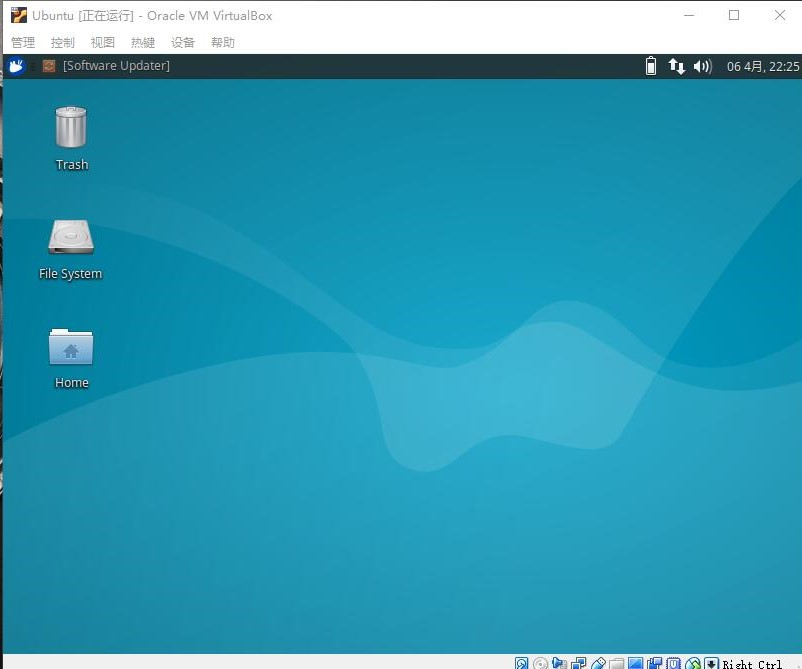
\includegraphics[width= 0.7\textwidth]{./fig/1_interface.jpg}
		\caption{The Interface of Linux}
		\label{fig:interface}
	\end{figure}
\end{minipage}
\begin{minipage}{0.5\textwidth}
	\begin{figure}[H]
		\centering
		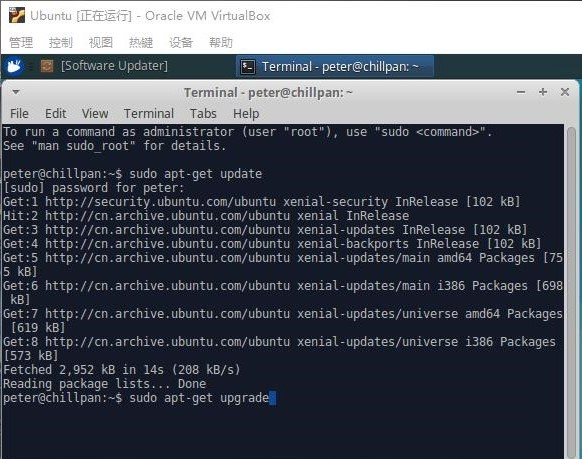
\includegraphics[width= 0.7\textwidth]{./fig/2_upgrade}
		\caption{Get Update and Upgrade}
		\label{fig:get update}
	\end{figure}
\end{minipage}

\par \quad \quad

2. Then we need to install gcc and other relevant supporting tools by :

\begin{lstlisting}[language = C]
 apt-get install gcc 
 apt-get install python-pip python-dev libffi-dev libssl-dev libxml2-dev libxslt1-dev zlibig-dev
 apt-get install 
\end{lstlisting}

\begin{minipage}{0.5\textwidth}
	\begin{figure}[H]
		\centering
		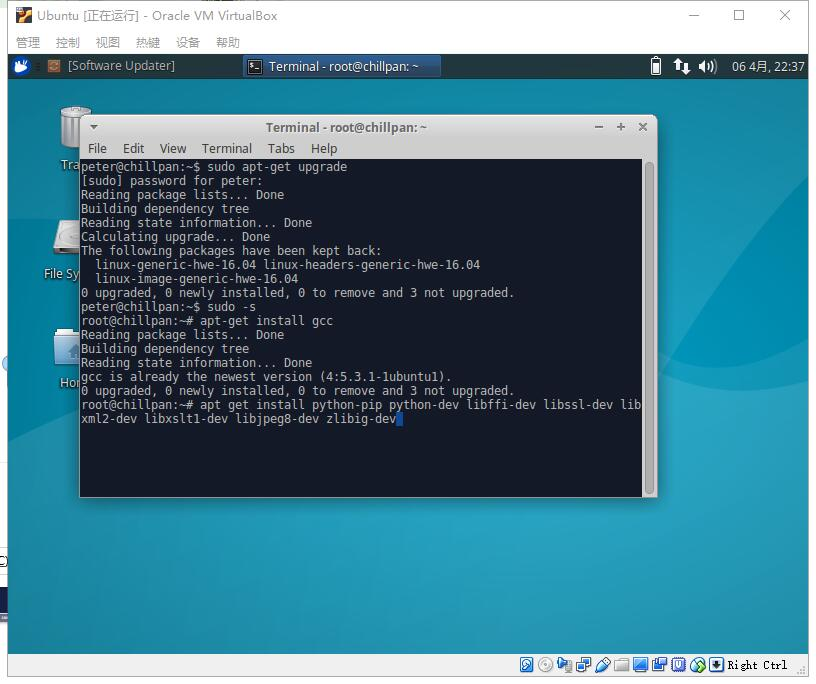
\includegraphics[width= 0.7\textwidth]{./fig/3_install_gcc_python.jpg}
		\caption{Install Supporting Tools}
		\label{fig:install gcc }
	\end{figure}
\end{minipage}
\begin{minipage}{0.5\textwidth}
	\begin{figure}[H]
		\centering
		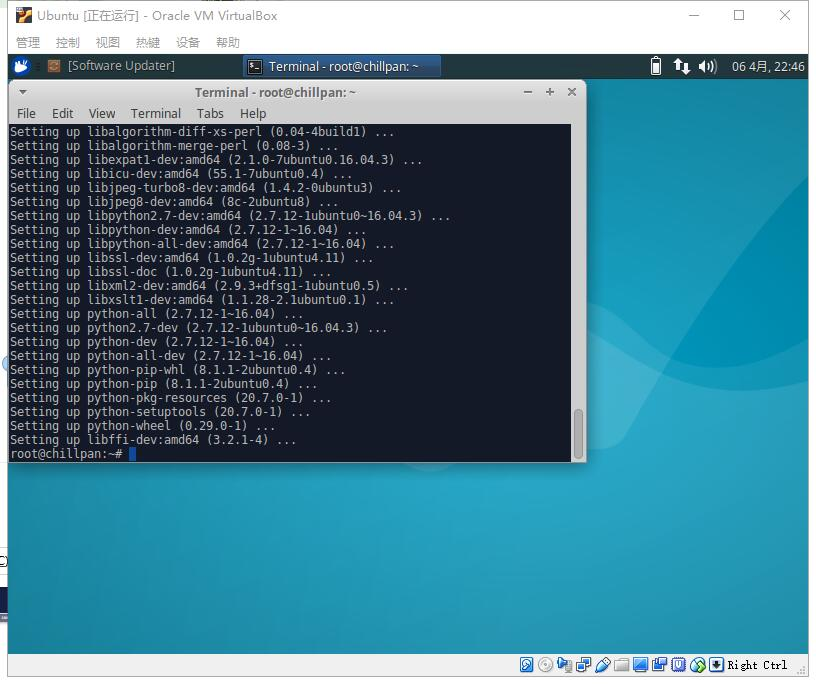
\includegraphics[width= 0.7\textwidth]{./fig/3_install_gcc_python_2.jpg}
		\caption{Get Install Finished}
		\label{fig:install gcc finished}
	\end{figure}
\end{minipage}

\subsection{Downloading the Kernel}
Then we need to download the kernel from {\color{blue}\url{http://www.kernel.org}} and unzip it by:

\begin{lstlisting}[language = C]
  wget wwww.kernel.org/pub/linux/kernel/v4.x/linux-4.10.13.tar.gz
  sudo -s  
  tar -xvf linux-4.10.13.tar.gz /usr/src/  
      //decompress file and move it to /usr/src/ 
\end{lstlisting}

\begin{minipage}{0.5\textwidth}
	\begin{figure}[H]
		\centering
		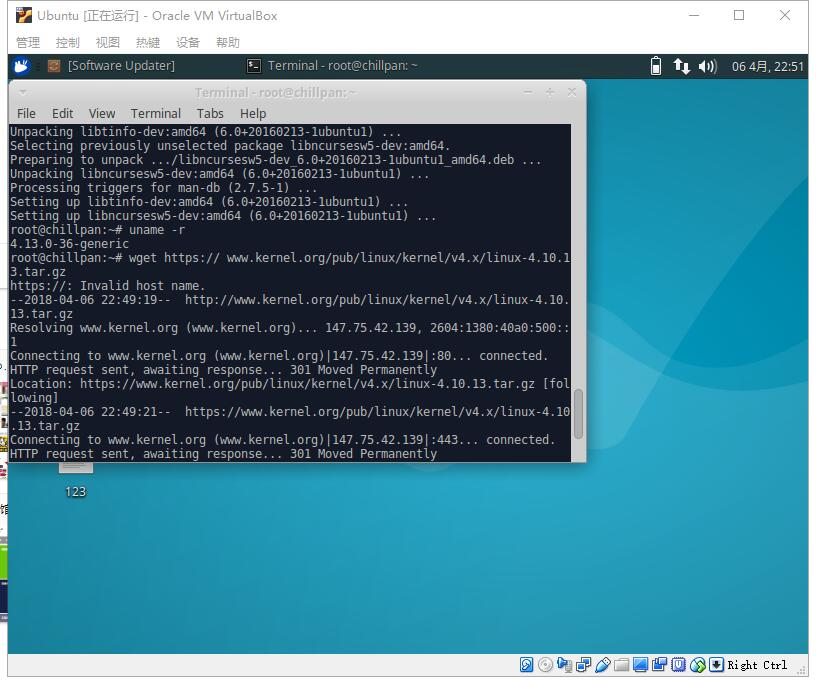
\includegraphics[width= 0.7\textwidth]{./fig/4_download_kernel.jpg}
		\caption{Download the Kernel}
		\label{fig:download kernel }
	\end{figure}
\end{minipage}
\begin{minipage}{0.5\textwidth}
	\begin{figure}[H]
		\centering
		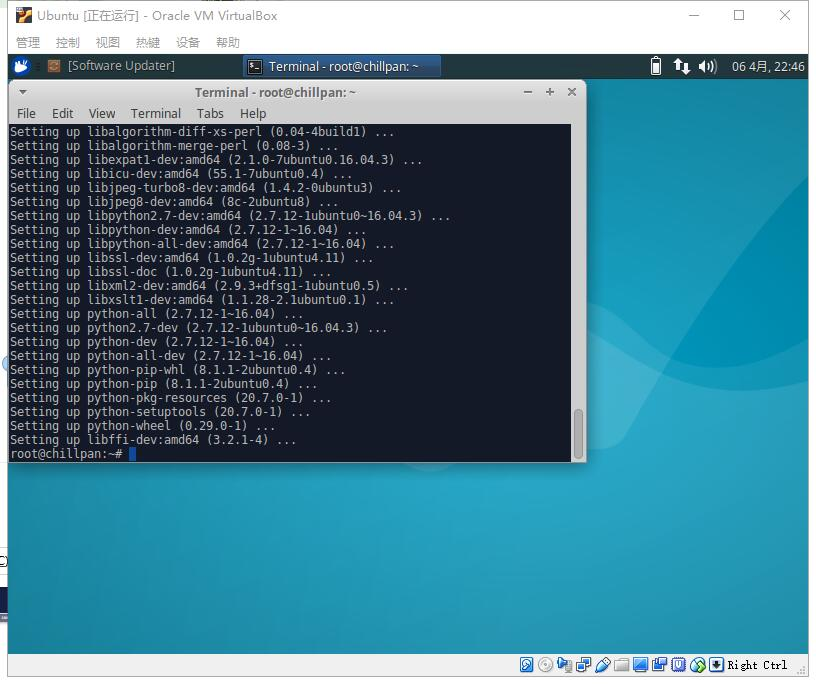
\includegraphics[width= 0.7\textwidth]{./fig/3_install_gcc_python_2.jpg}
		\caption{Unzip the Kernel}
		\label{fig:unzip kernel}
	\end{figure}
\end{minipage}

\subsection{Create Helloworld File}
1. We create a helloworld folder in "/usr/src/linux-4.10.13" and generate file "helloworld.c"
\begin{lstlisting}[language = C]
 /usr/src/linux-4.10.13 mkdir helloworld
 /usr/src/linux-4.10.13 cd helloworld
 /usr/src/linux-4.10.13/helloworld gedit helloworld.c
\end{lstlisting}

2. The code for "helloword.c" is: 

\begin{lstlisting}[language = C]
#include <linux/kernel.h>

asmlinkage long sys_helloworld(void){
      printk("Hello world\n");
      return 0;
}
\end{lstlisting}

3. Create corresponding MakeFile for this:

\begin{lstlisting}[language = C]
 gedit Makefile
       obj-y := helloworld.o
\end{lstlisting}

\begin{minipage}{0.5\textwidth}
	\begin{figure}[H]
		\centering
		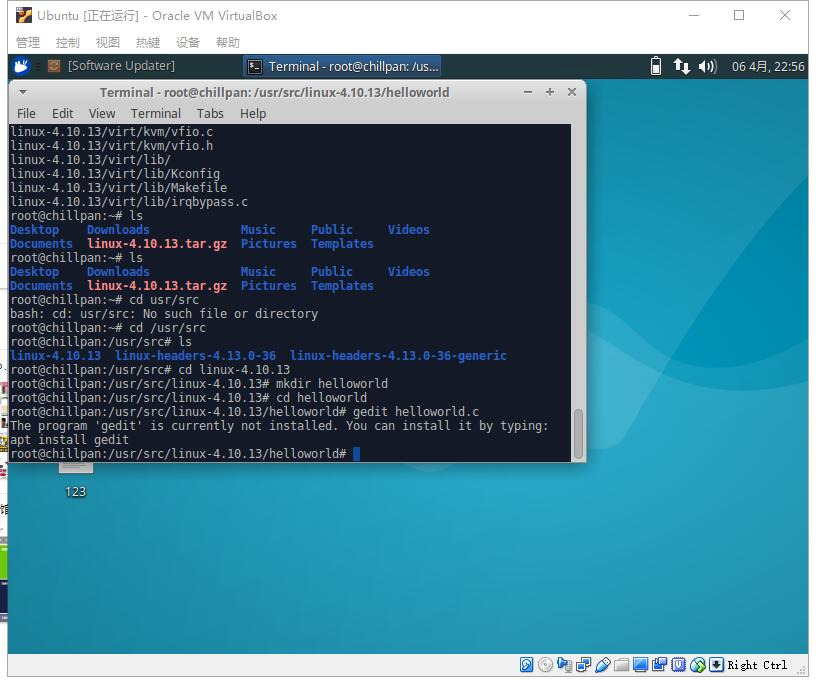
\includegraphics[width= 0.7\textwidth]{./fig/6_create_helloworld.jpg}
		\caption{Create Helloworld Folder and File}
		\label{fig:create helloworld }
	\end{figure}
\end{minipage}
\begin{minipage}{0.5\textwidth}
	\begin{figure}[H]
		\centering
		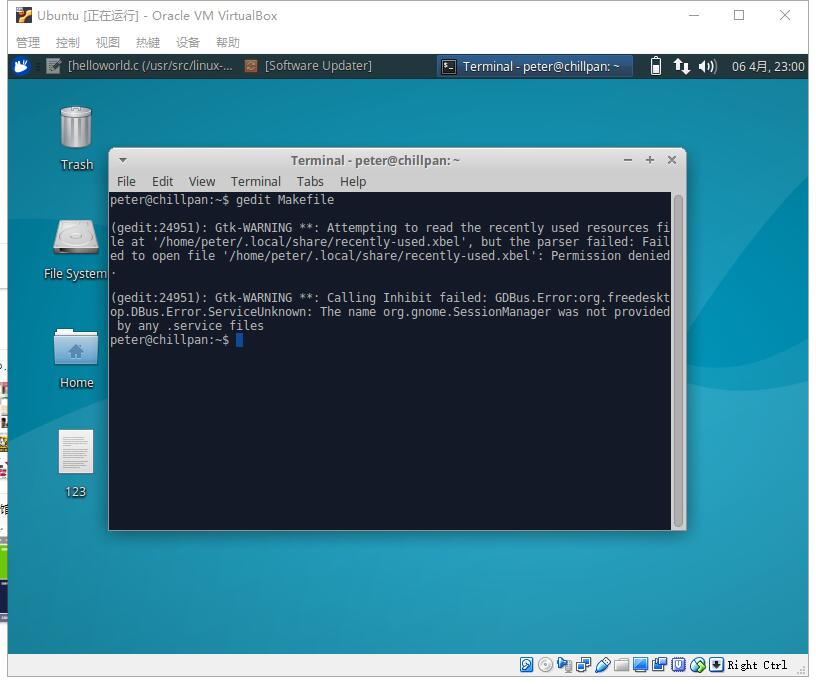
\includegraphics[width= 0.7\textwidth]{./fig/7_make_file.jpg}
		\caption{MakeFile}
		\label{fig: make file}
	\end{figure}
\end{minipage}

\par \quad 
\par \quad 

4. Then we have to change it in the Makefile for Linux Kernel:

	\begin{figure}[H]
	\centering
	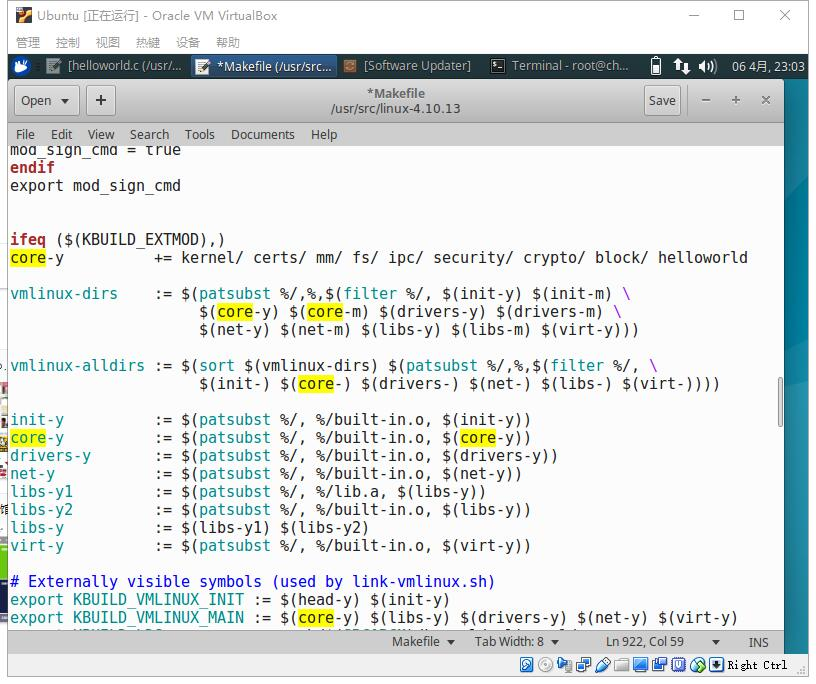
\includegraphics[width= 0.6\textwidth]{./fig/8_addto_Makefile.jpg}
	\caption{Add to MakeFile for Linux Kernel}
	\label{fig:linux kernel make file}
    \end{figure}

\subsection{Add Helloworld to System Calls}
Open syscalls.h and add helloword:

\begin{lstlisting}[language = C]
  cd include/linux
  gedit syscalls.h
  
  asmlinkage long sys_helloworld(void);
  
\end{lstlisting}

\begin{minipage}{0.5\textwidth}
	\begin{figure}[H]
		\centering
		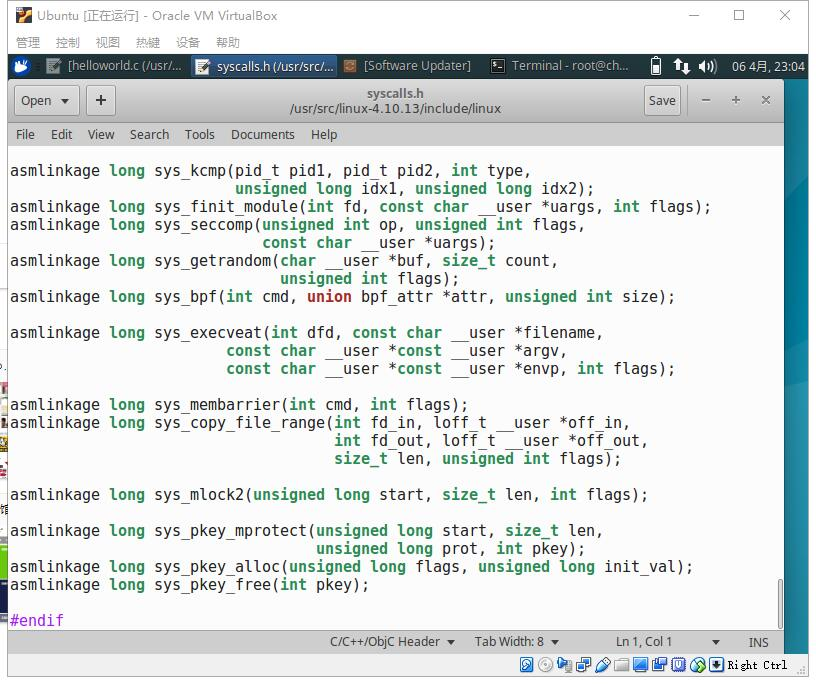
\includegraphics[width= 0.7\textwidth]{./fig/9_addto_syscalls.jpg}
		\caption{The System Calls Before}
		\label{fig:systemcalls before}
	\end{figure}
\end{minipage}
\begin{minipage}{0.5\textwidth}
	\begin{figure}[H]
		\centering
		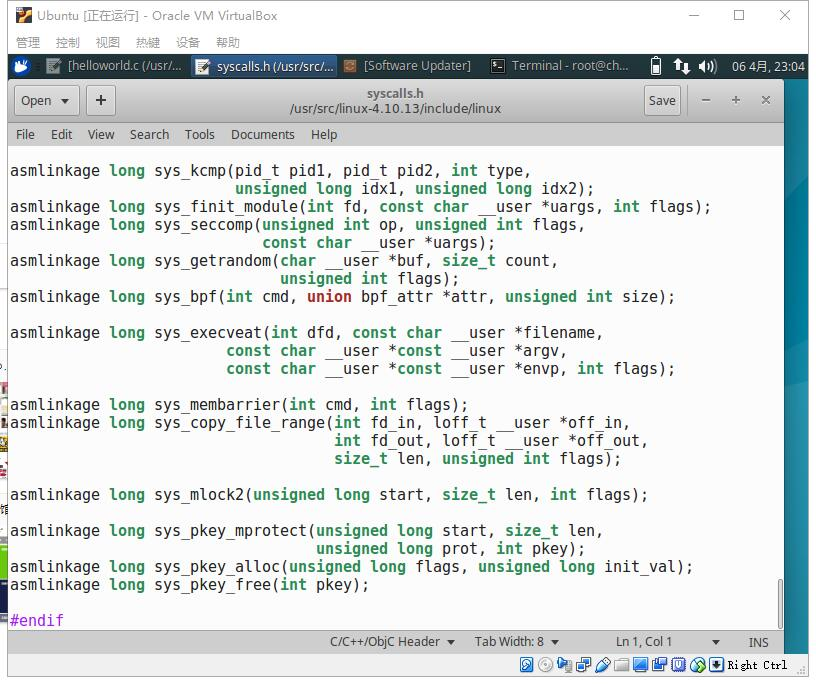
\includegraphics[width= 0.7\textwidth]{./fig/9_addto_syscalls.jpg}
		\caption{The System Calls After}
		\label{fig: systemcalls after}
	\end{figure}
\end{minipage}

\subsection{Modify the Pointer List}

1. Get it the folder for syscalls' .tbl:
\begin{lstlisting}[language = C]
  cd /usr/src/linux-4.10.13/arch/x86/entry/syscalls
  gedit syscall_64.tbl
\end{lstlisting}

2. Add another systemcalls and record its number \textbf{332}
\begin{lstlisting}[language = C]
  332    64     helloworld     sys_helloworld
\end{lstlisting}

\begin{minipage}{0.5\textwidth}
	\begin{figure}[H]
		\centering
		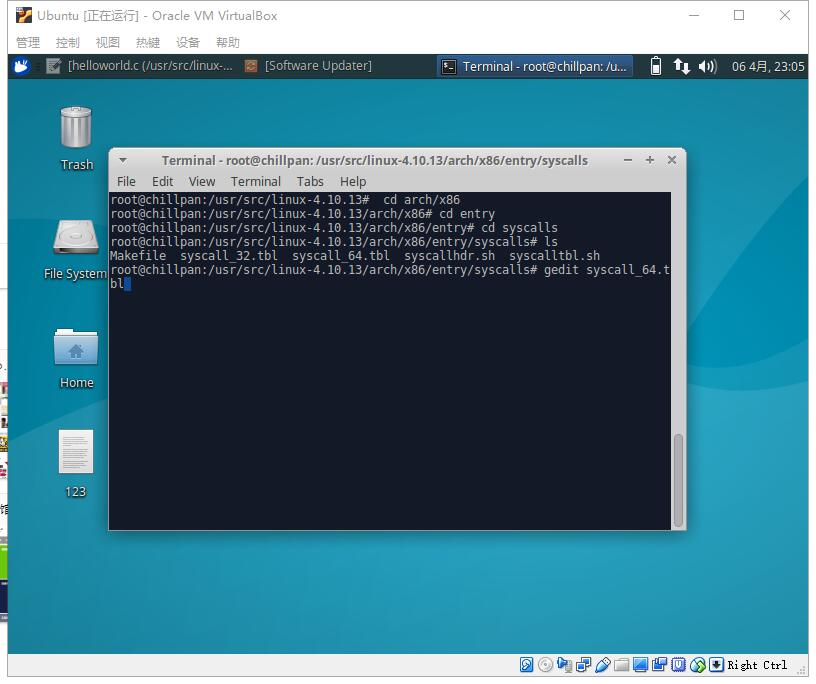
\includegraphics[width= 0.7\textwidth]{./fig/10_syscall_64_tbl.jpg}
		\caption{Get into Syscall's .tbl Folder}
	\end{figure}
\end{minipage}
\begin{minipage}{0.5\textwidth}
	\begin{figure}[H]
		\centering
		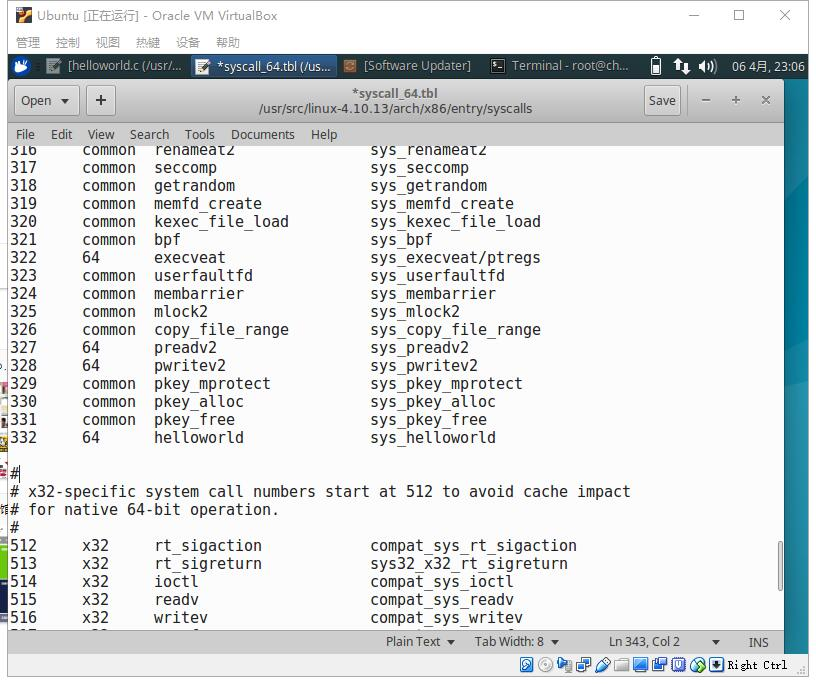
\includegraphics[width= 0.7\textwidth]{./fig/11_syscall_helloworld_entry.jpg}
		\caption{Add Helloworld as System Call \textbf{332}}
	\end{figure}
\end{minipage}

\subsection{Compile the Kernel}

1. We make the relevant configuration by make menuconfig:
\begin{lstlisting}[language = C]
  make menuconfig 
  make oldconfig
\end{lstlisting}

\begin{minipage}{0.5\textwidth}
\begin{figure}[H]
	\centering
	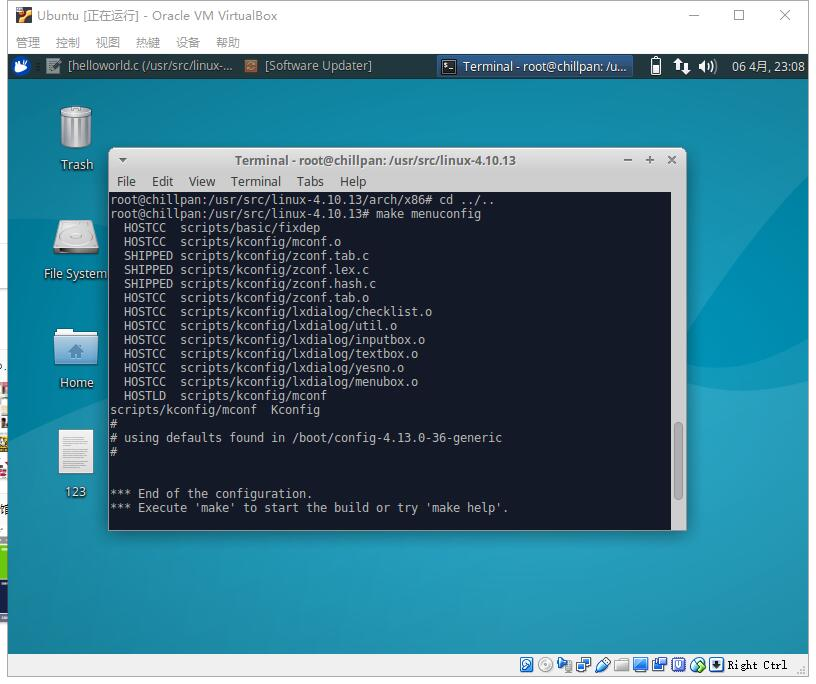
\includegraphics[width= 0.7\textwidth]{./fig/12_menuconfig.jpg}
	\caption{Make Menuconfig}
\end{figure}
\end{minipage}
\begin{minipage}{0.5\textwidth}
\begin{figure}[H]
	\centering
	\includegraphics[width= 0.7\textwidth]{./fig/12_menuconfig_2.jpg}
	\caption{The Menu}
\end{figure}
\end{minipage}

2. Then we compile the kernel and consumes about 2 hours:
\begin{lstlisting}[language = C]
   /usr/src/linux-4.10.13#  make 
   scripts/kconfig/conf  -slientoldconfig kconfig
       SYSTBL  arch/x86/entry/syscalls/../../include/generated/asm/syscalls_32.h
       SYSTBL  arch/x86/entry/syscalls/../../include/generated/asm/syscalls_32.h
       SYSHDR  arch/x86/entry/syscalls/../../include/generated/asm/unistd_ia32.h
       SYSHDR  arch/x86/entry/syscalls/../../include/generated/asm/unistd_x32.h
       /*
       The compiling of related functions and else
       ...
       ...
       /*
\end{lstlisting}

\subsection{Install the Kernel}

1. Install the kernel

\begin{lstlisting}[language = C]
  make modules_install
  make install
\end{lstlisting}

2. Make new kernel to be loaded

\begin{lstlisting}[language = C]
  sudo mkinitramfs -o /boot/initrd.img-4.10.13
  sudo update  -initramfs -c -k -4.10.13
  sudo update  -grub2
\end{lstlisting}

3. Add choice to the grup list

\begin{lstlisting}[language = C]
  sudo update  -grub2
\end{lstlisting}

\begin{minipage}{0.5\textwidth}
	\begin{figure}[H]
		\centering
		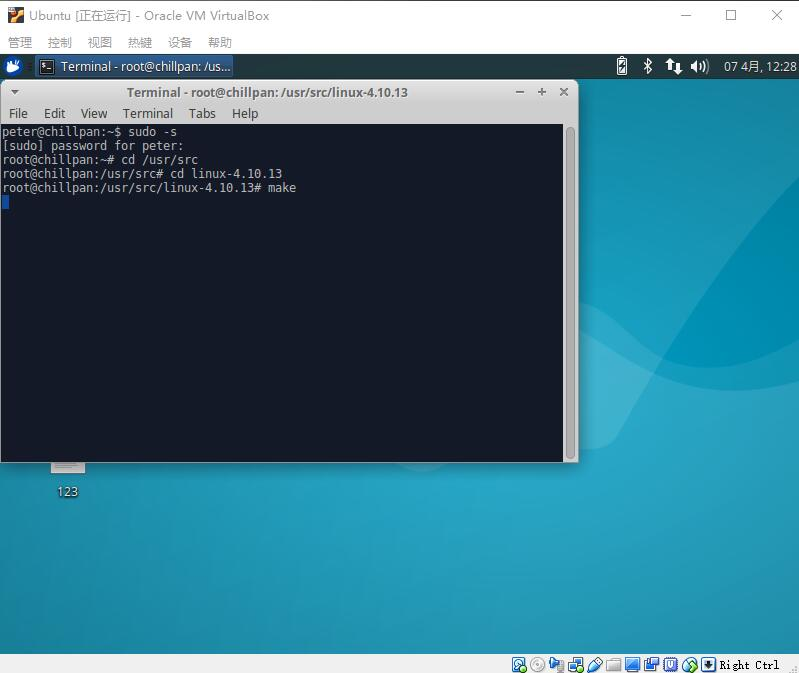
\includegraphics[width= 0.7\textwidth]{./fig/13_make.jpg}
	\end{figure}
\end{minipage}
\begin{minipage}{0.5\textwidth}
	\begin{figure}[H]
		\centering
		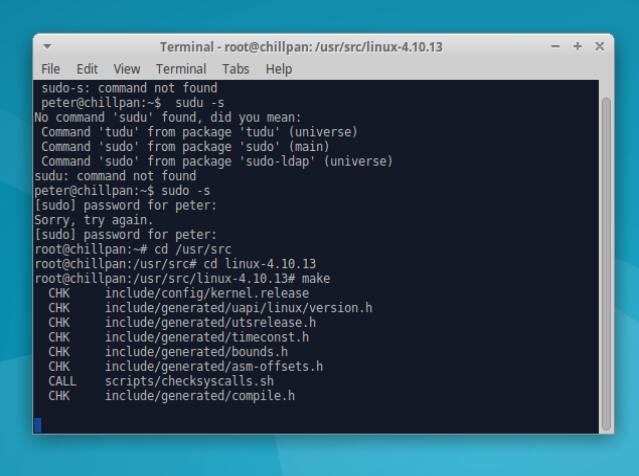
\includegraphics[width= 0.7\textwidth]{./fig/make.jpg}
	\end{figure}
\end{minipage}
\begin{figure}[H]
	\centering
	\caption{Make}
\end{figure}

\subsection{Reboot}
1. Reboot the ubuntu and choose to enter the 4.10.13 version kernel. Check if we successfully change the kernel:

\begin{lstlisting}[language = C]
   uname -r
\end{lstlisting}

2. Write a program to use System Call 332

\begin{lstlisting}[language = C]
#include<stdio.h>
#include<unistd.h>
#include<sys/syscall.h>

#define SYS_Helloworld   332  
//same as defined before

int main(){
   long int s = syscall(SYS_Helloworld);
   printf("System call : sys_helloworld returned %li \n",s);
   for (int i = 0 ; i < 10 ; i++)
     syscall(SYS_Helloworld);
   return 0;
}

\end{lstlisting}

\section{Project Result}

The result for programs before returns 0, which means that sys\_helloworld has been successfully called.

Use \textbf{dmesg} to examine:

\begin{lstlisting}[language = C]
  peter@chillpan: ~/Desktop$ dmesg
\end{lstlisting}

\begin{minipage}{0.5\textwidth}
	\begin{figure}[H]
		\centering
		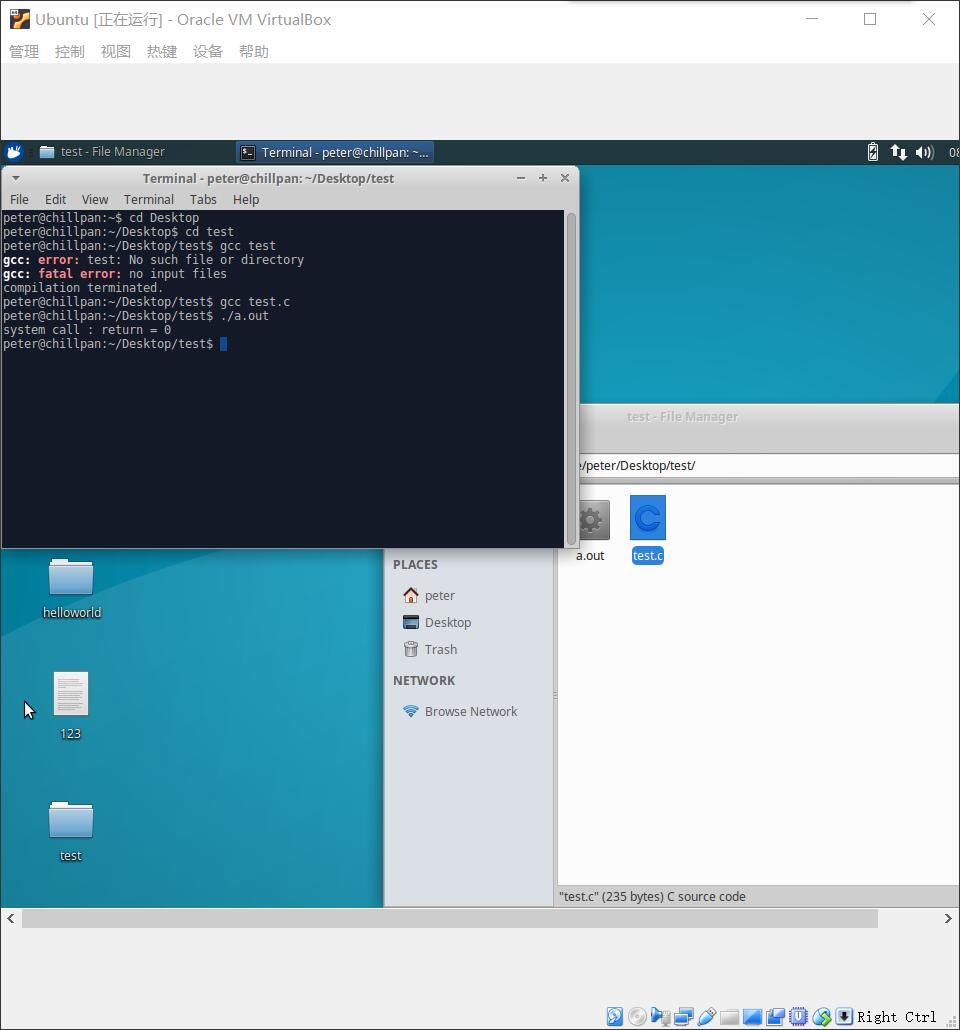
\includegraphics[width= 0.7\textwidth]{./fig/15_running.jpg}
	\end{figure}
\end{minipage}
\begin{minipage}{0.5\textwidth}
	\begin{figure}[H]
		\centering
		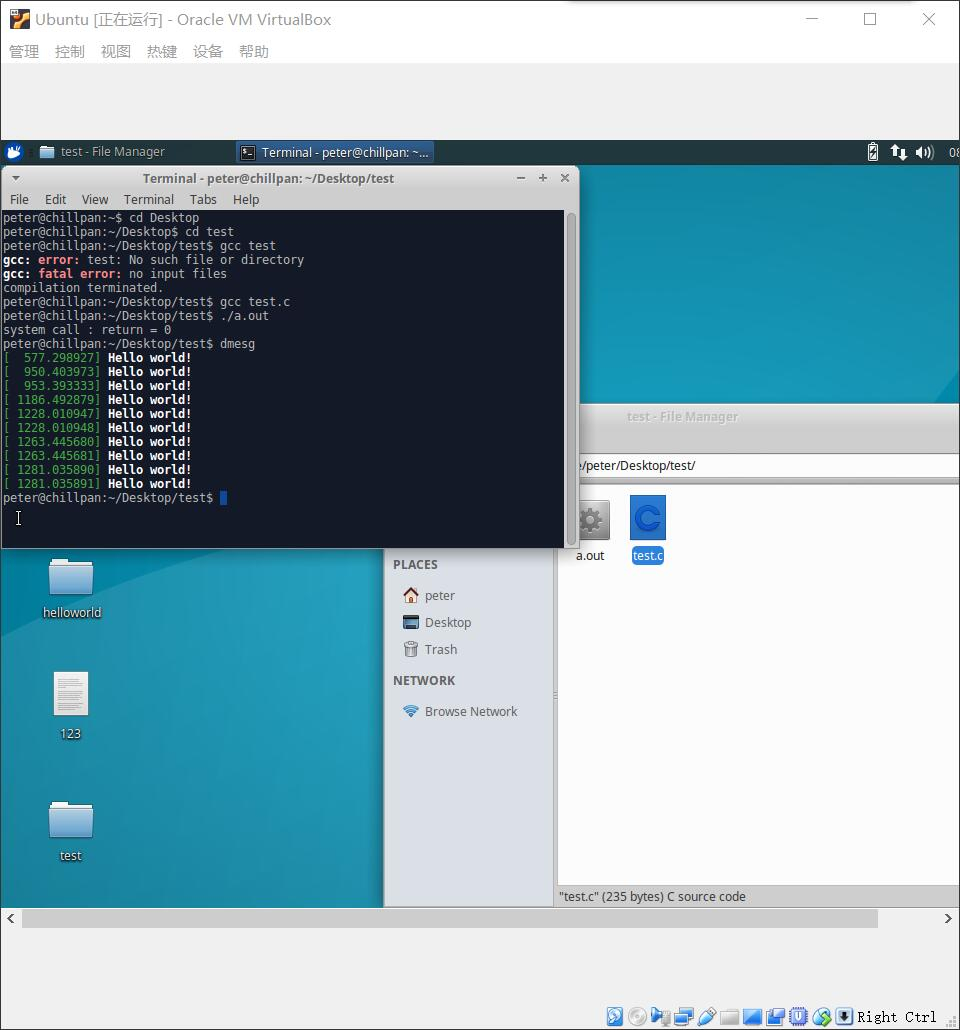
\includegraphics[width= 0.7\textwidth]{./fig/16_helloworld.jpg}
	\end{figure}
\end{minipage}
\begin{figure}[H]
	\centering
	\caption{Project Result}
\end{figure}

\section{Problem Conquered}

The most frustrating  problem is the following error:\\
     .size expression for apf\_fault does not evaluate to a constant.

\begin{figure}[H]
	\centering
	\includegraphics[width= 0.7\textwidth]{./fig/error1.jpg}
	\caption{Error}
\end{figure}

And at first I did not find this problem, because I was not using the command "make bzImage", then I found that the command "make -j4" runs very fast, which only needed about 10 minutes, much shorter than my room mates. Later I found I can’t "make install".

\begin{figure}[H]
	\centering
	\includegraphics[width= 0.7\textwidth]{./fig/error2.jpg}
	\caption{Error: can not make install}
\end{figure}

So I think there must be something wrong, and I searched the website to find more command to try, until I tried the "make bzImage" command to find the problem.

Fortunately, there’s someone having solved this problem\footnote{\url{http://blog.csdn.net/baozhb/article/details/9005150}}. 

The solution is to modify two lines of codes (code mistake) in /.../arch/x86/kernel/entry\_32.S. And then the problem is solved quickly.


\section{Harvest}

Through this project I learned a lot knowledge about the kernel and how to add a system call. Although I haven’t done as the same as what the book recommend, but I think my way is as good too, which is more simple. The operating system is a very fun thing to manipulate, and solving problems makes me very proudable.


\end{document}
